% Created by tikzDevice version 0.10.1 on 2016-04-19 18:05:50
% !TEX encoding = UTF-8 Unicode
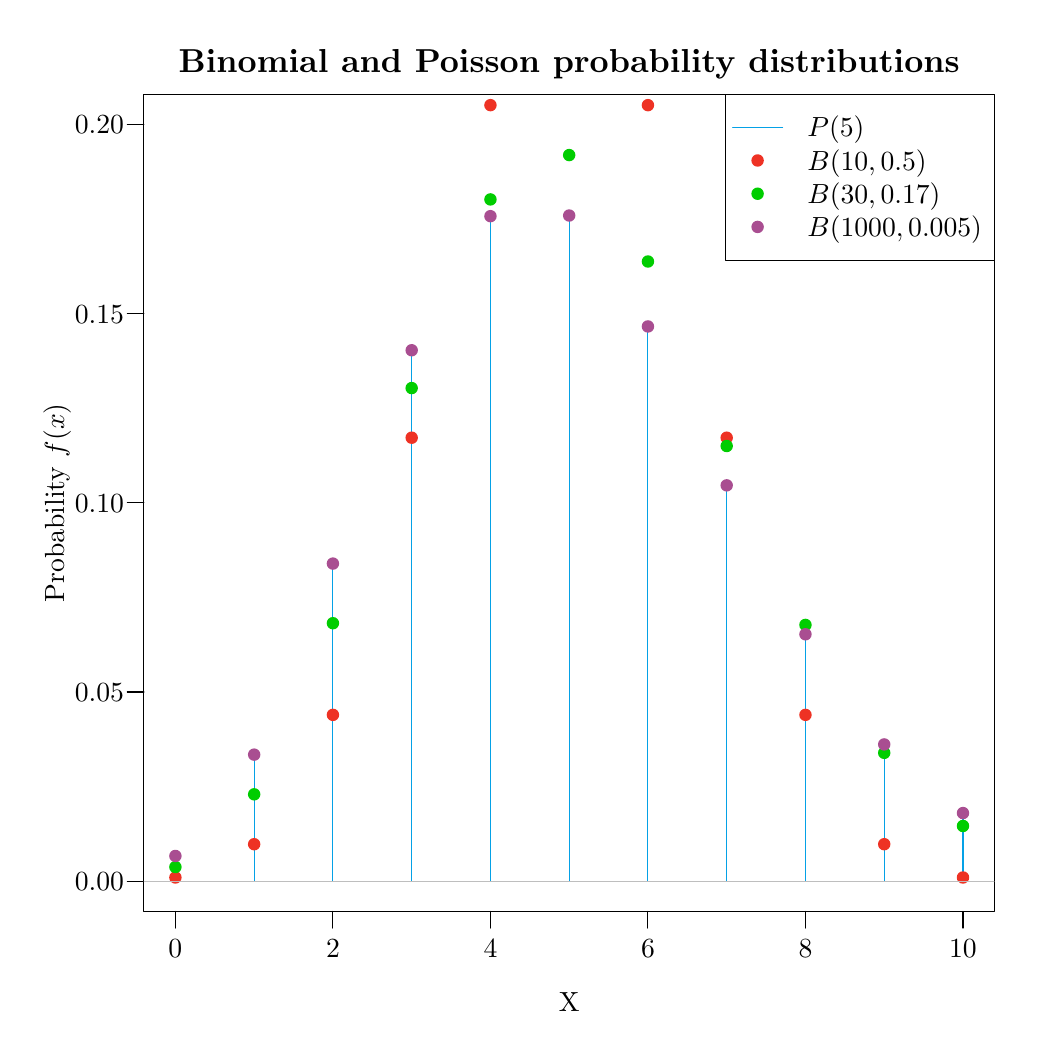
\begin{tikzpicture}[x=1pt,y=1pt]
\definecolor{fillColor}{RGB}{255,255,255}
\path[use as bounding box,fill=fillColor,fill opacity=0.00] (0,0) rectangle (361.35,361.35);
\begin{scope}
\path[clip] ( 42.00, 42.00) rectangle (349.35,337.35);
\definecolor{drawColor}{RGB}{5,161,230}

\path[draw=drawColor,line width= 0.4pt,line join=round,line cap=round] ( 53.38, 52.94) -- ( 53.38, 62.15);

\path[draw=drawColor,line width= 0.4pt,line join=round,line cap=round] ( 81.84, 52.94) -- ( 81.84, 99.00);

\path[draw=drawColor,line width= 0.4pt,line join=round,line cap=round] (110.30, 52.94) -- (110.30,168.10);

\path[draw=drawColor,line width= 0.4pt,line join=round,line cap=round] (138.76, 52.94) -- (138.76,244.88);

\path[draw=drawColor,line width= 0.4pt,line join=round,line cap=round] (167.22, 52.94) -- (167.22,292.87);

\path[draw=drawColor,line width= 0.4pt,line join=round,line cap=round] (195.67, 52.94) -- (195.67,292.87);

\path[draw=drawColor,line width= 0.4pt,line join=round,line cap=round] (224.13, 52.94) -- (224.13,252.88);

\path[draw=drawColor,line width= 0.4pt,line join=round,line cap=round] (252.59, 52.94) -- (252.59,195.75);

\path[draw=drawColor,line width= 0.4pt,line join=round,line cap=round] (281.05, 52.94) -- (281.05,142.20);

\path[draw=drawColor,line width= 0.4pt,line join=round,line cap=round] (309.51, 52.94) -- (309.51,102.53);

\path[draw=drawColor,line width= 0.4pt,line join=round,line cap=round] (337.97, 52.94) -- (337.97, 77.73);
\end{scope}
\begin{scope}
\path[clip] (  0.00,  0.00) rectangle (361.35,361.35);
\definecolor{drawColor}{RGB}{0,0,0}

\path[draw=drawColor,line width= 0.4pt,line join=round,line cap=round] ( 53.38, 42.00) -- (337.97, 42.00);

\path[draw=drawColor,line width= 0.4pt,line join=round,line cap=round] ( 53.38, 42.00) -- ( 53.38, 36.00);

\path[draw=drawColor,line width= 0.4pt,line join=round,line cap=round] (110.30, 42.00) -- (110.30, 36.00);

\path[draw=drawColor,line width= 0.4pt,line join=round,line cap=round] (167.22, 42.00) -- (167.22, 36.00);

\path[draw=drawColor,line width= 0.4pt,line join=round,line cap=round] (224.13, 42.00) -- (224.13, 36.00);

\path[draw=drawColor,line width= 0.4pt,line join=round,line cap=round] (281.05, 42.00) -- (281.05, 36.00);

\path[draw=drawColor,line width= 0.4pt,line join=round,line cap=round] (337.97, 42.00) -- (337.97, 36.00);

\node[text=drawColor,anchor=base,inner sep=0pt, outer sep=0pt, scale=  1.00] at ( 53.38, 25.20) {0};

\node[text=drawColor,anchor=base,inner sep=0pt, outer sep=0pt, scale=  1.00] at (110.30, 25.20) {2};

\node[text=drawColor,anchor=base,inner sep=0pt, outer sep=0pt, scale=  1.00] at (167.22, 25.20) {4};

\node[text=drawColor,anchor=base,inner sep=0pt, outer sep=0pt, scale=  1.00] at (224.13, 25.20) {6};

\node[text=drawColor,anchor=base,inner sep=0pt, outer sep=0pt, scale=  1.00] at (281.05, 25.20) {8};

\node[text=drawColor,anchor=base,inner sep=0pt, outer sep=0pt, scale=  1.00] at (337.97, 25.20) {10};

\path[draw=drawColor,line width= 0.4pt,line join=round,line cap=round] ( 42.00, 52.94) -- ( 42.00,326.41);

\path[draw=drawColor,line width= 0.4pt,line join=round,line cap=round] ( 42.00, 52.94) -- ( 36.00, 52.94);

\path[draw=drawColor,line width= 0.4pt,line join=round,line cap=round] ( 42.00,121.31) -- ( 36.00,121.31);

\path[draw=drawColor,line width= 0.4pt,line join=round,line cap=round] ( 42.00,189.67) -- ( 36.00,189.67);

\path[draw=drawColor,line width= 0.4pt,line join=round,line cap=round] ( 42.00,258.04) -- ( 36.00,258.04);

\path[draw=drawColor,line width= 0.4pt,line join=round,line cap=round] ( 42.00,326.41) -- ( 36.00,326.41);

\node[text=drawColor,anchor=base east,inner sep=0pt, outer sep=0pt, scale=  1.00] at ( 34.80, 49.49) {0.00};

\node[text=drawColor,anchor=base east,inner sep=0pt, outer sep=0pt, scale=  1.00] at ( 34.80,117.86) {0.05};

\node[text=drawColor,anchor=base east,inner sep=0pt, outer sep=0pt, scale=  1.00] at ( 34.80,186.23) {0.10};

\node[text=drawColor,anchor=base east,inner sep=0pt, outer sep=0pt, scale=  1.00] at ( 34.80,254.60) {0.15};

\node[text=drawColor,anchor=base east,inner sep=0pt, outer sep=0pt, scale=  1.00] at ( 34.80,322.97) {0.20};

\path[draw=drawColor,line width= 0.4pt,line join=round,line cap=round] ( 42.00, 42.00) --
	(349.35, 42.00) --
	(349.35,337.35) --
	( 42.00,337.35) --
	( 42.00, 42.00);
\end{scope}
\begin{scope}
\path[clip] (  0.00,  0.00) rectangle (361.35,361.35);
\definecolor{drawColor}{RGB}{0,0,0}

\node[text=drawColor,anchor=base,inner sep=0pt, outer sep=0pt, scale=  1.20] at (195.67,345.16) {\bfseries Binomial and Poisson probability distributions};

\node[text=drawColor,anchor=base,inner sep=0pt, outer sep=0pt, scale=  1.00] at (195.67,  6.00) {X};

\node[text=drawColor,rotate= 90.00,anchor=base,inner sep=0pt, outer sep=0pt, scale=  1.00] at ( 13.20,189.67) {Probability $f(x)$};
\end{scope}
\begin{scope}
\path[clip] ( 42.00, 42.00) rectangle (349.35,337.35);
\definecolor{fillColor}{RGB}{238,50,36}

\path[fill=fillColor] ( 53.38, 54.27) circle (  2.25);

\path[fill=fillColor] ( 81.84, 66.29) circle (  2.25);

\path[fill=fillColor] (110.30,113.03) circle (  2.25);

\path[fill=fillColor] (138.76,213.18) circle (  2.25);

\path[fill=fillColor] (167.22,333.35) circle (  2.25);

\path[fill=fillColor] (224.13,333.35) circle (  2.25);

\path[fill=fillColor] (252.59,213.18) circle (  2.25);

\path[fill=fillColor] (281.05,113.03) circle (  2.25);

\path[fill=fillColor] (309.51, 66.29) circle (  2.25);

\path[fill=fillColor] (337.97, 54.27) circle (  2.25);
\definecolor{fillColor}{RGB}{0,205,0}

\path[fill=fillColor] ( 53.38, 58.05) circle (  2.25);

\path[fill=fillColor] ( 81.84, 84.32) circle (  2.25);

\path[fill=fillColor] (110.30,146.15) circle (  2.25);

\path[fill=fillColor] (138.76,231.12) circle (  2.25);

\path[fill=fillColor] (167.22,299.28) circle (  2.25);

\path[fill=fillColor] (195.67,315.31) circle (  2.25);

\path[fill=fillColor] (224.13,276.85) circle (  2.25);

\path[fill=fillColor] (252.59,210.18) circle (  2.25);

\path[fill=fillColor] (281.05,145.53) circle (  2.25);

\path[fill=fillColor] (309.51, 99.30) circle (  2.25);

\path[fill=fillColor] (337.97, 72.88) circle (  2.25);
\definecolor{fillColor}{RGB}{169,78,145}

\path[fill=fillColor] ( 53.38, 62.04) circle (  2.25);

\path[fill=fillColor] ( 81.84, 98.66) circle (  2.25);

\path[fill=fillColor] (110.30,167.70) circle (  2.25);

\path[fill=fillColor] (138.76,244.78) circle (  2.25);

\path[fill=fillColor] (167.22,293.23) circle (  2.25);

\path[fill=fillColor] (195.67,293.47) circle (  2.25);

\path[fill=fillColor] (224.13,253.38) circle (  2.25);

\path[fill=fillColor] (252.59,195.97) circle (  2.25);

\path[fill=fillColor] (281.05,142.15) circle (  2.25);

\path[fill=fillColor] (309.51,102.35) circle (  2.25);

\path[fill=fillColor] (337.97, 77.55) circle (  2.25);
\definecolor{drawColor}{RGB}{190,190,190}

\path[draw=drawColor,line width= 0.4pt,line join=round,line cap=round] ( 42.00, 52.94) -- (349.35, 52.94);
\definecolor{drawColor}{RGB}{0,0,0}

\path[draw=drawColor,line width= 0.4pt,line join=round,line cap=round] (252.06,337.35) rectangle (349.35,277.35);
\definecolor{drawColor}{RGB}{5,161,230}

\path[draw=drawColor,line width= 0.4pt,line join=round,line cap=round] (254.76,325.35) -- (272.76,325.35);
\definecolor{fillColor}{RGB}{238,50,36}

\path[fill=fillColor] (263.76,313.35) circle (  2.25);
\definecolor{fillColor}{RGB}{0,205,0}

\path[fill=fillColor] (263.76,301.35) circle (  2.25);
\definecolor{fillColor}{RGB}{169,78,145}

\path[fill=fillColor] (263.76,289.35) circle (  2.25);
\definecolor{drawColor}{RGB}{0,0,0}

\node[text=drawColor,anchor=base west,inner sep=0pt, outer sep=0pt, scale=  1.00] at (281.76,321.91) {$P(5)$};

\node[text=drawColor,anchor=base west,inner sep=0pt, outer sep=0pt, scale=  1.00] at (281.76,309.91) {$B(10,0.5)$};

\node[text=drawColor,anchor=base west,inner sep=0pt, outer sep=0pt, scale=  1.00] at (281.76,297.91) {$B(30,0.17)$};

\node[text=drawColor,anchor=base west,inner sep=0pt, outer sep=0pt, scale=  1.00] at (281.76,285.91) {$B(1000,0.005)$};
\end{scope}
\end{tikzpicture}
